\begin{figure}[ht]
  \centering
  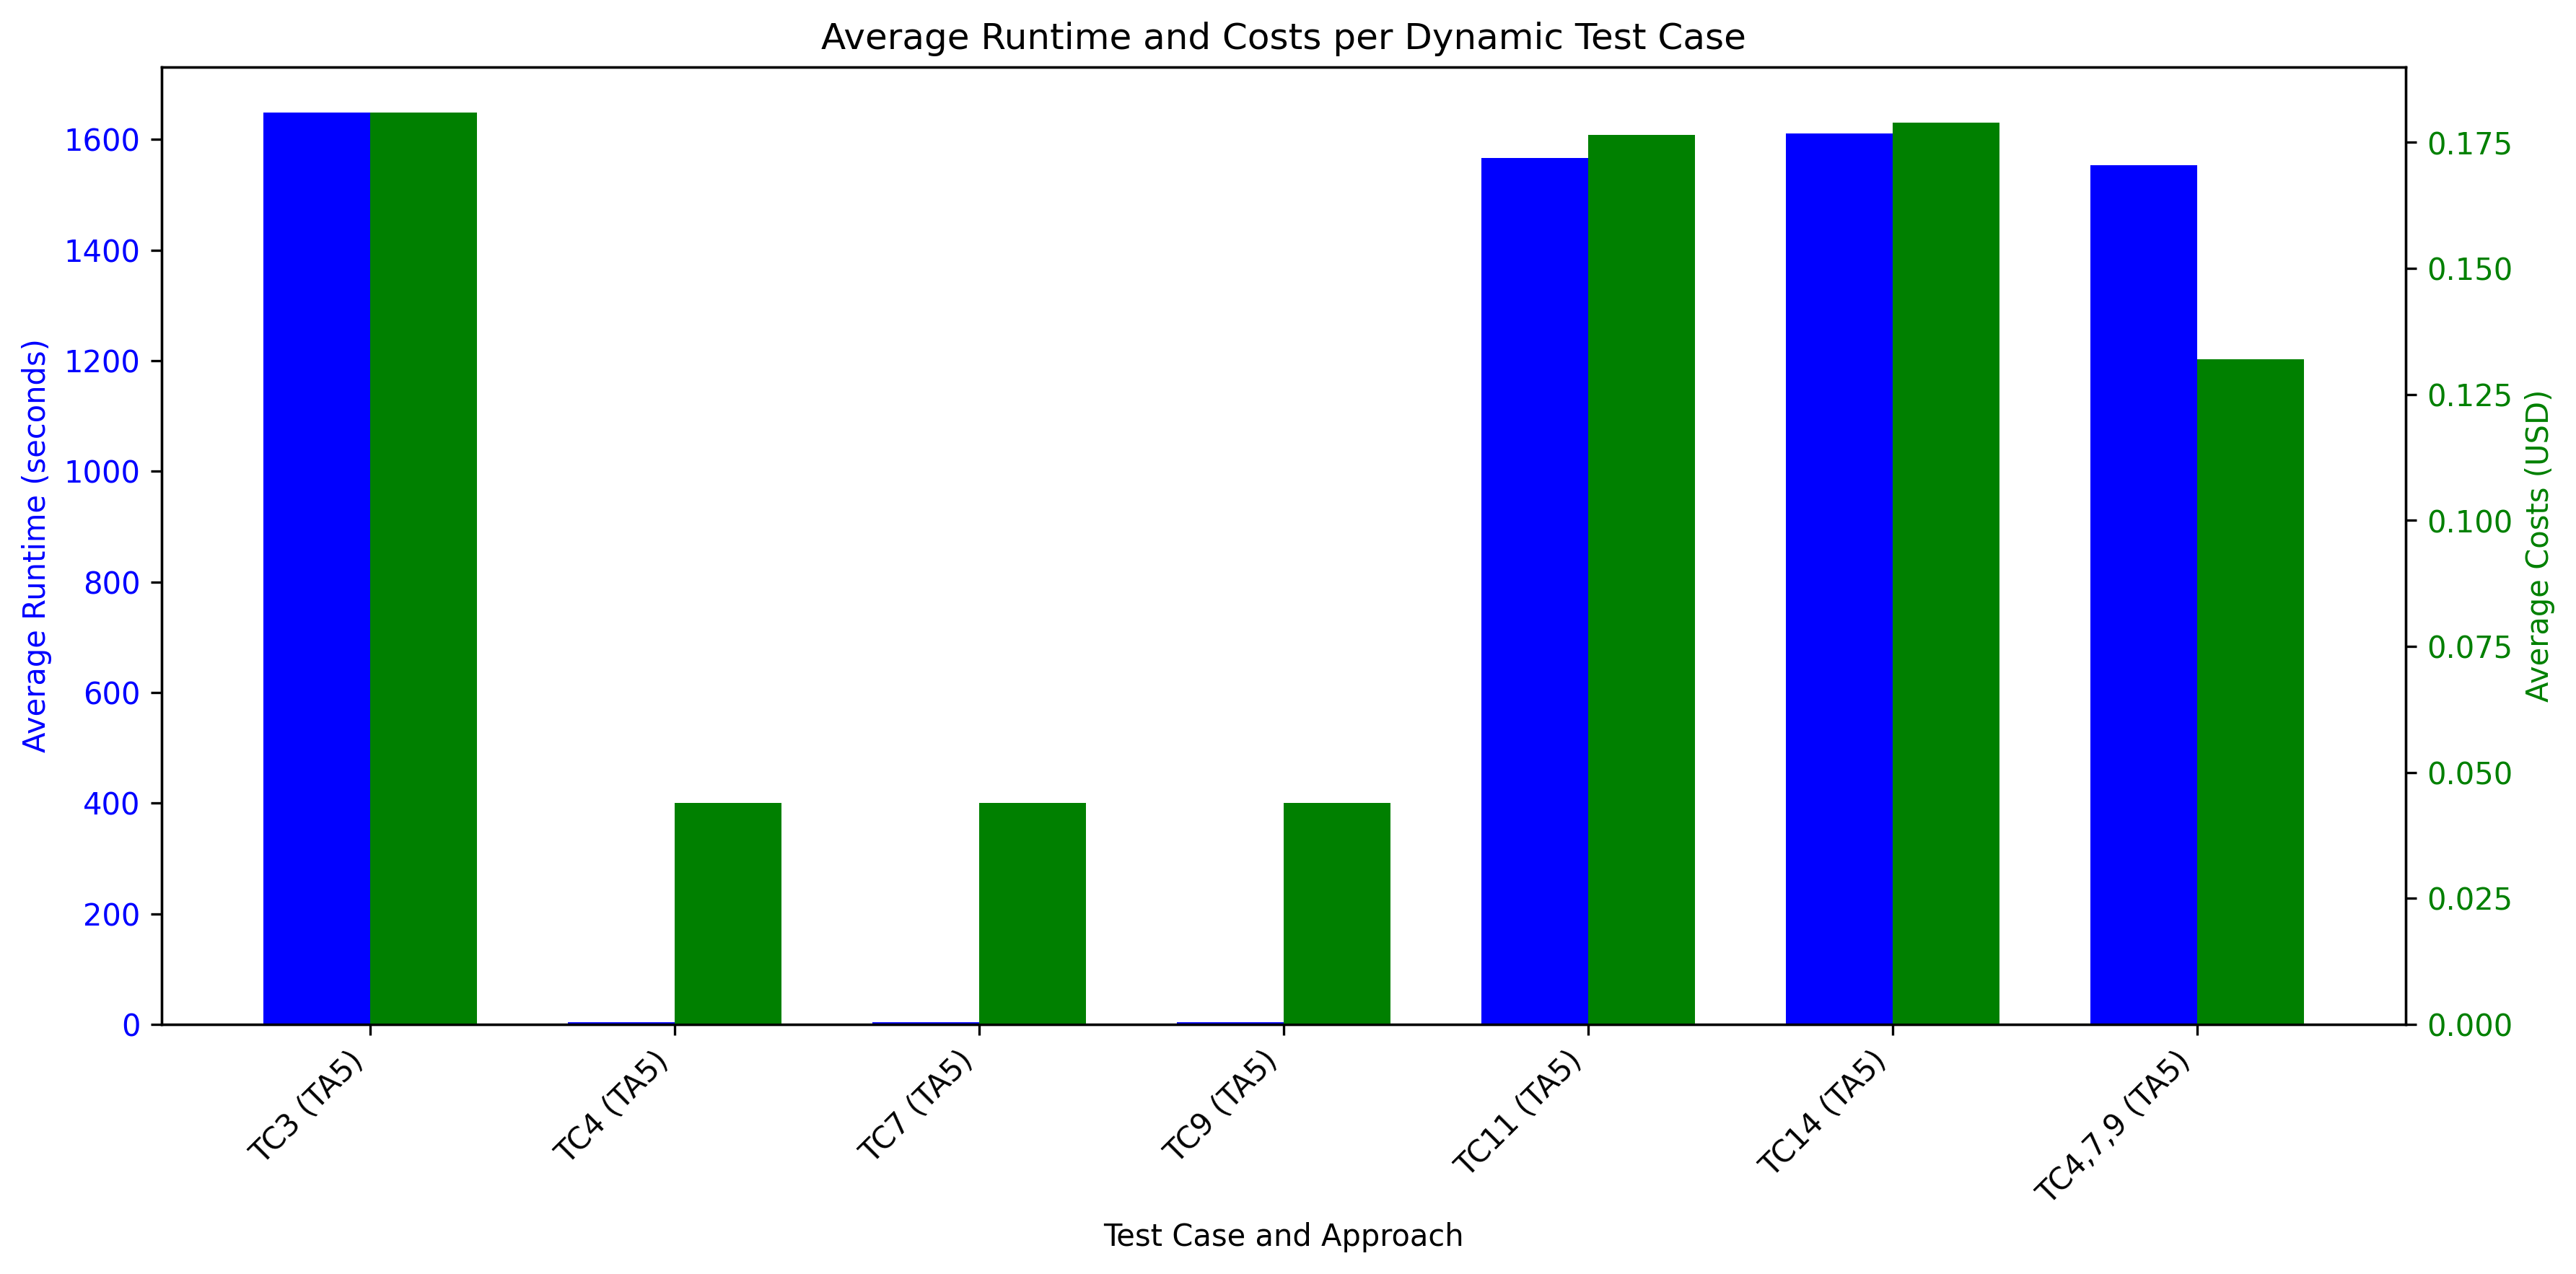
\includegraphics[width=\textwidth]{img/tc_avg_runtime_and_cost.png}
  \caption{Average Runtime and Costs per Dynamic Test Case}
  \label{fig:tc_avg_runtime_and_cost}
\end{figure}

\begin{table}[h!]
  \begin{tabular}{|l | l | l|}
    \hline
    \textbf{Test Case and Approach} & \textbf{Average Runtime (seconds)} & \textbf{Average Costs (USD)} \\
    \hline
    TC3 (TA5) & 1648.35 & 0.18092 \\
    \hline
    TC4 (TA5) & 3.7619 & 0.044 \\
    \hline
    TC7 (TA5) & 3.38095 & 0.04398 \\
    \hline
    TC9 (TA5) & 3.66667 & 0.04399 \\
    \hline
    TC11 (TA5) & 1566.04762 & 0.17649 \\
    \hline
    TC14 (TA5) & 1610.36364 & 0.17887 \\
    \hline
    TC4,7,9 (TA5) & 1553.80952 & 0.13197 \\
    \hline
  \end{tabular}
  \caption{Average Runtime and Costs per Dynamic Test Case}
  \label{tab:tc_avg_runtime_and_cost}
\end{table}
